\documentclass[aspectratio=169]{beamer}

\mode<presentation>
{
  \usetheme{default}
  \usecolortheme{seahorse}
  \usefonttheme{professionalfonts}
  \setbeamertemplate{navigation symbols}{}
  \setbeamertemplate{caption}[numbered]
  \setbeamertemplate{footline}[frame number]
}

\usepackage[utf8x]{inputenc}
\usepackage{graphicx}
\usepackage{physics}
\usepackage{caption}
\usepackage{subcaption}
\usepackage{xcolor}
\usepackage{physics}
\usepackage{amsmath}
\usepackage{tikz}
\usetikzlibrary{positioning}
\usepackage{mathdots}
\usepackage{yhmath}
\usepackage{cancel}
\usepackage{color}
\usepackage{siunitx}
\usepackage{array}
\usepackage{multirow}
\usepackage{amssymb}
\usepackage{gensymb}
\usepackage{tabularx}
\usepackage{extarrows}
\usepackage{booktabs}
\usepackage{centernot}


\title{Online tuning of storage ring non-linear dynamics at SIRIUS and fast ORM measurement}

\author{Matheus Melo Santos Velloso \\{\small MSc. student}}

\institute{Gleb Wataghin Institute of Physics - University of Campinas\\ Accelerator Physics Group (FAC) -  Brazilian Syncrhotron Laboratory (LNLS)}

\date{Optics Tuning and Corrections for Future Colliders Workshop \\ CERN, June 2023}

\AtBeginSection[]
{
    \begin{frame}[noframenumbering,plain]
         \tableofcontents[currentsection]
   \end{frame}
}

\begin{document}
{
\setbeamertemplate{background}
{
    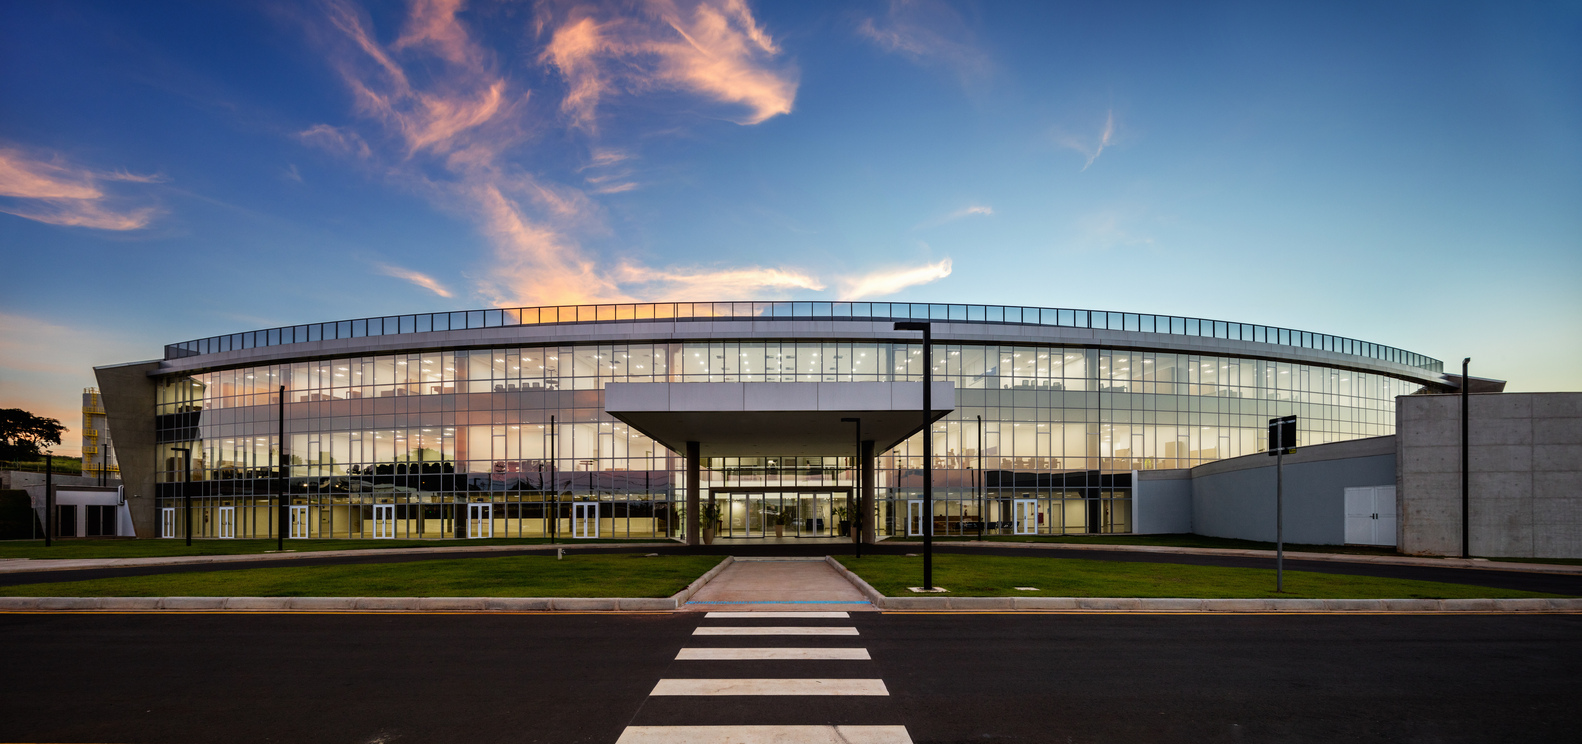
\includegraphics[width=\paperwidth, height=\paperheight]{sirius.jpg}
}
\begin{frame}[plain]
    % Title & Subtitle
    \begin{tikzpicture}[remember picture, overlay]
        \node
        [
            above=2.5cm,
            align=center,
            fill=white!20,
            inner xsep=15pt,
            inner ysep=10pt,
            minimum width=0.9\textwidth,
            text width=0.9\textwidth
        ] (title) at (current page.center)
        {
            \LARGE Online Tuning of Storage Ring Nonlinear Dynamics  \\[5pt]
            \small and Fast ORM Measruement at SIRIUS
        };

        \node[below = 0.4cm, align=center] at (title.south) 
        {            
        Optics Tuning and Corrections for Future Colliders Workshop \\[2pt]
        CERN, June 27, 2023
        };
    
        % Author
        \node
        [
            above left= 0.2cm and 0cm,
            align=right,
        ] (author) at (current page.south east)
        {
            \scriptsize \textcolor{white}{Matheus M. S. Velloso}  \\
            \tiny \textcolor{white}{Brazilian Synchrotron Laboratory (LNLS/CNPEM)} \\
            \tiny \textcolor{white}{Gleb Wataghin Institute of Physics (IFGW/UNICAMP)} \\
            \scriptsize \textcolor{white}{on behalf of the LNLS Accelerator Physics Group}
        };

        \node
        [
            above right =0.2cm and 0.2cm
        ] at (current page.south west)
        {
            
\includegraphics[width=3.5cm]{cnpem_lnls.png}
        };

    \end{tikzpicture}
\end{frame}
}
% \begin{frame}{Contents}
%     \tableofcontents
% \end{frame}

\section{Introduction}
\begin{frame}{SIRIUS storage ring}
    \begin{minipage}{0.35\textwidth}
        \begin{figure}
            \centering
            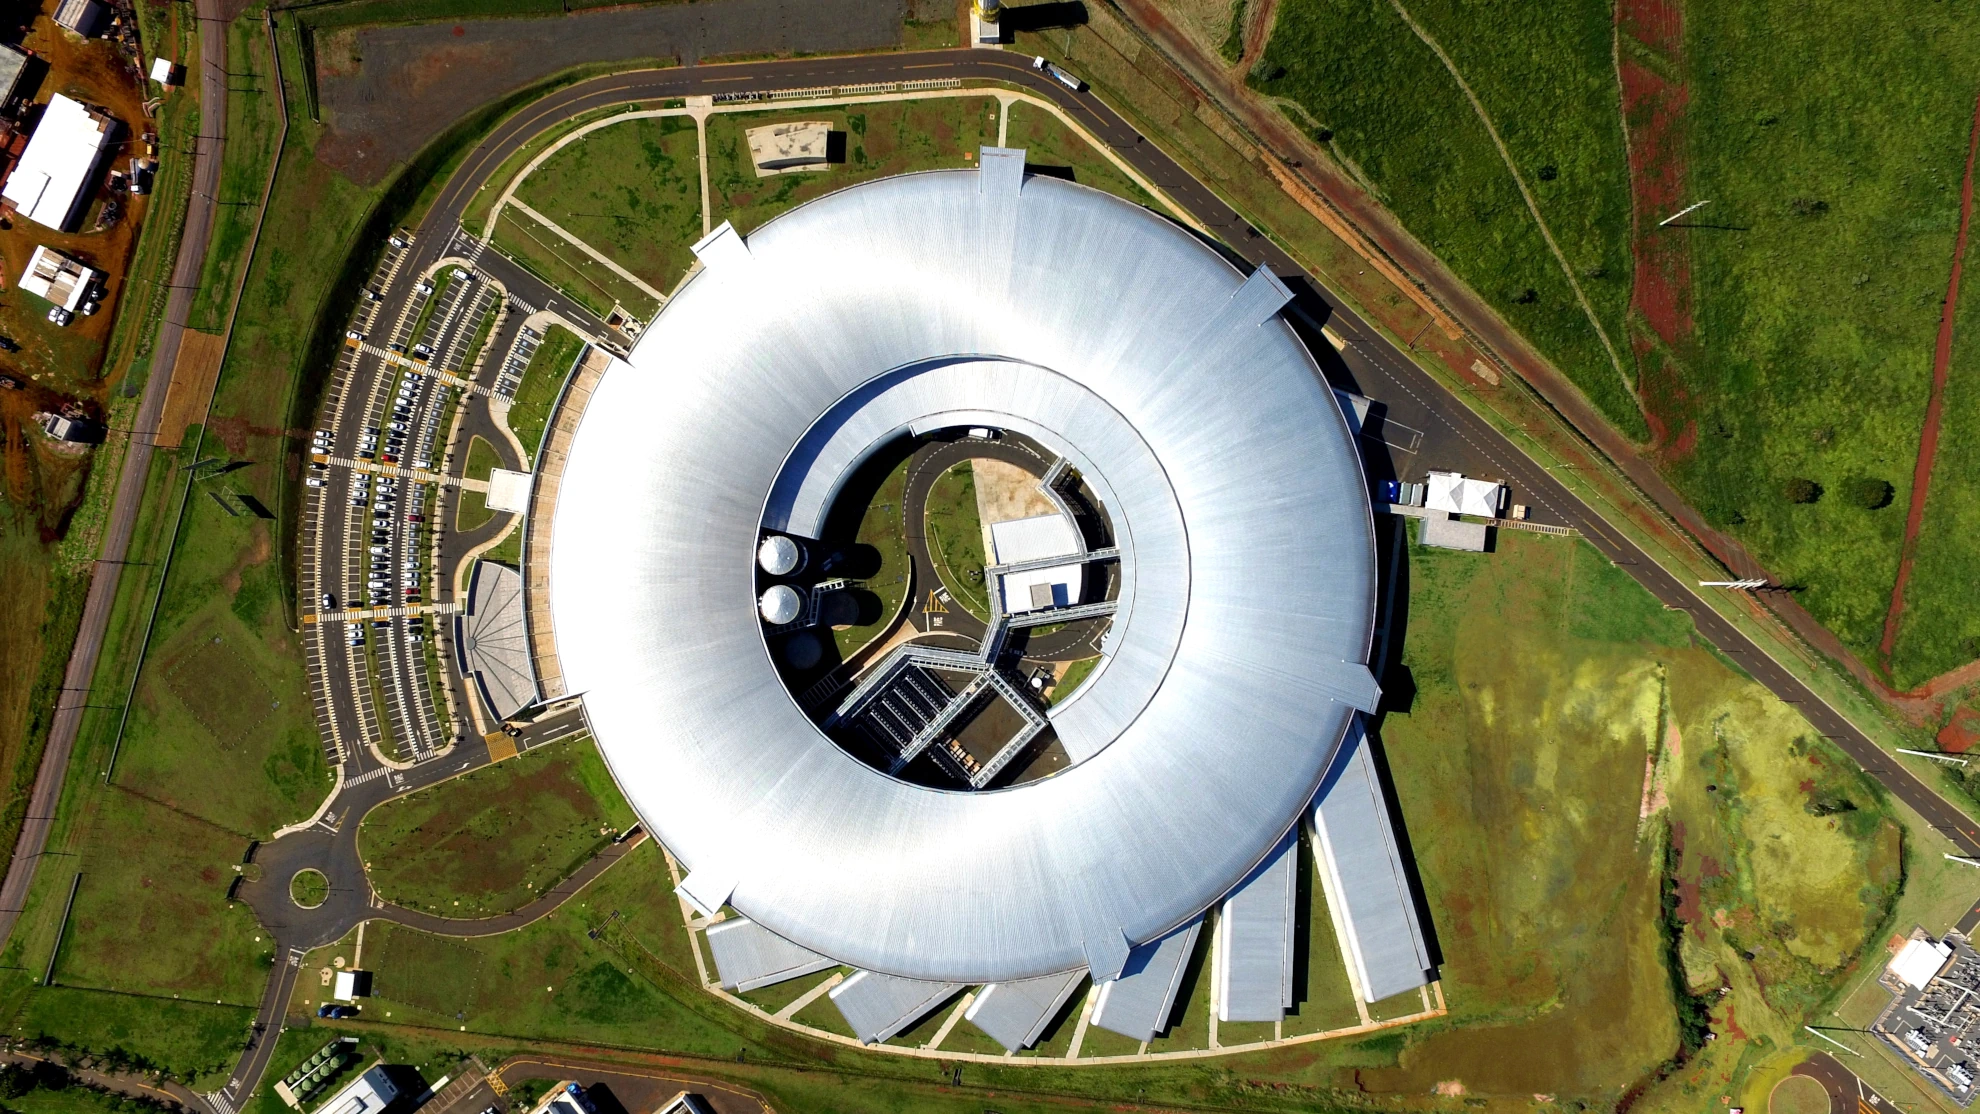
\includegraphics[angle=90, width=0.7\textwidth]{f1.png}
        \end{figure}
    \end{minipage}
    \hfill
    \begin{minipage}{0.62\textwidth}
        \scriptsize
        Designed, built and operated by the Brazilian Synchrotron Laboratory (LNLS), at the Brazilian Center for Research in Energy and Materials (CNPEM) campus, at Campinas, Brazil.\\

        \begin{tabular}{lccc}
                \toprule\toprule
                Parameter & & Currently & Phase I \\
                \toprule
                Energy  & $E_0$  & $\SI{3}{\giga\electronvolt}$ & \\
                Current & $I_0$ &  $\SI{100}{\milli\ampere}$ & $\SI{350}{\milli\ampere}$ \\
                Operation mode & & Top-up &      \\
                RF Cavities & & 1 NC & 2 SC + HC \\
                RF Voltage & $\hat{V}_{\mathrm{rf}}$ &  $\SI{1.5}{\mega\volt}$ & $\SI{3.0}{\mega\volt}$\\
                RF Frequency &   $f_{\mathrm{rf}}$ &  $\SI{499.667}{\mega\hertz}$ &  \\
                Harmonic Number &   $h$ &  864 \\
                Momentum compaction factor & $\alpha$ &   $\SI{1.6e-4}{}$ & \\
                Energy Spread & $\sigma_\delta$ &  $\SI{8.5e-4}{}$ & \\
                Bunch length & $\sigma_z$ &  $\SI{2.5}{\milli\meter}$ & $\SI{12}{\milli\meter}$ \\
                Energy loss p/ turn & $U_0$ &  $\SI{470}{\kilo\electronvolt}$ & $\SI{870}{\kilo\electronvolt}$ \\
                Lifetime & $\tau$ & $\SI{15}{\hour}$ & $>\SI{10}{\hour}$ \\
                % Synchrotron Tune & $\nu_z$ & $\SI{0.001638}{}$ \\
                % Frequência Síncrotron & $f_z$ &  $\SI{2.5}{\kilo\hertz}$ & \\
                % Amortecimento Longitudinal & $\tau_\delta$ &  $\SI{13}{\milli\second}$ & \\             % \\
                % \bottomrule
                % HC Type &  & Passive SC \\
                % HC RF harmonic & $q$ & 3 \\
                % HC Shunt Impedance & $R_s$ & $\SI{8.25}{\mega\ohm}$ \\
                % HC Quality Factor & $Q$ & $\SI{20800}{}$ \\
                % HC R/Q & $R/Q$ & $\SI{396}{\ohm}$ \\
                \bottomrule\bottomrule
        \end{tabular}
    \end{minipage}
\end{frame}

\begin{frame}{SIRIUS Lattice and Optics}
    20-cell 5BA lattice with 5-fold symmetric high (A) and low (B, P) betatron functions sections. Superperiod = A-B-P-B
    \begin{figure}
        \centering
        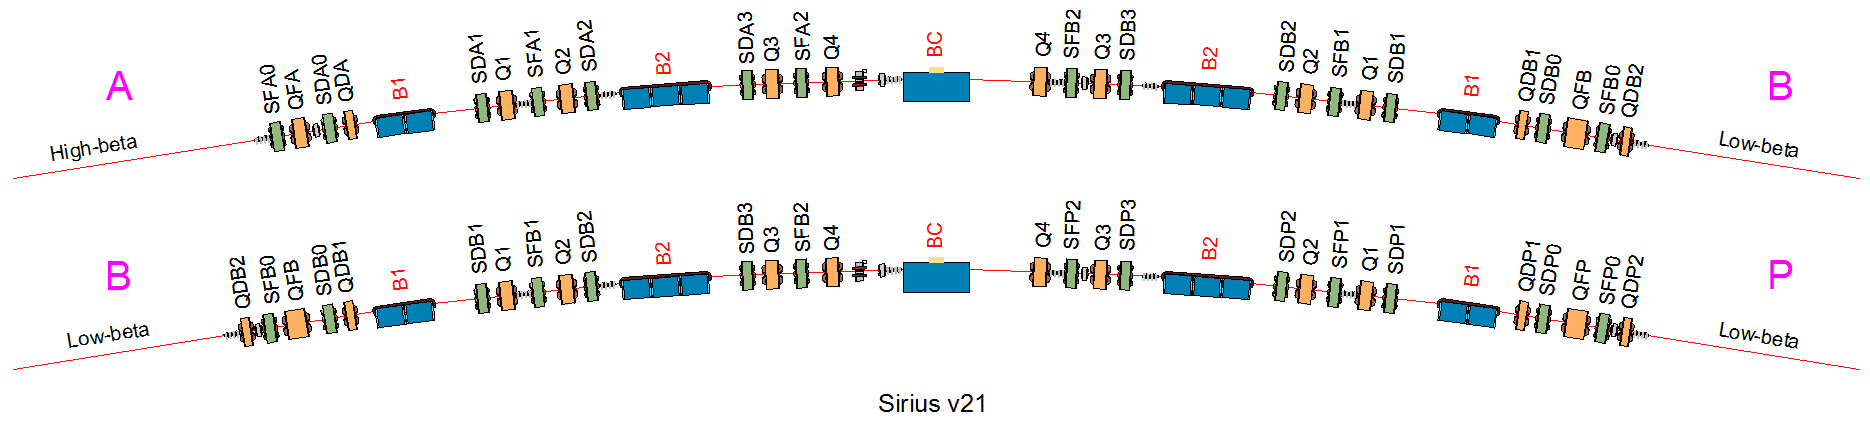
\includegraphics[width=0.8\textwidth]{SI_superperiod.png}
    \end{figure}
    \begin{figure}
        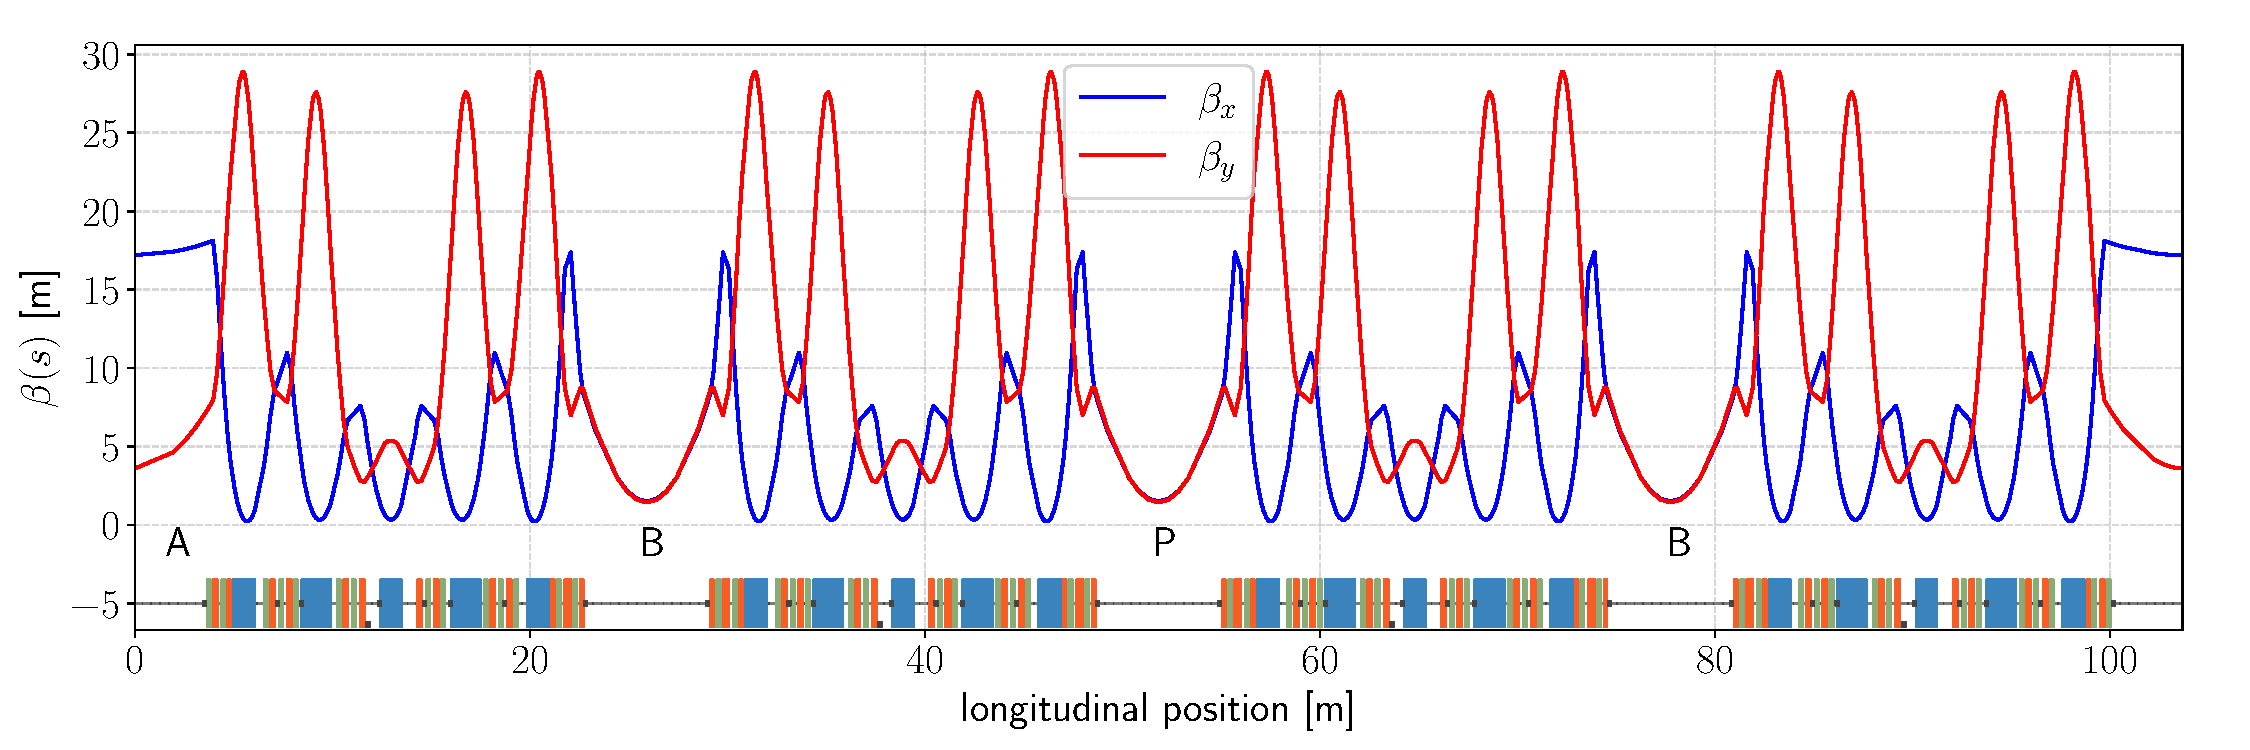
\includegraphics[width=0.8\textwidth]{beta_functions.pdf}
    \end{figure}
\end{frame}

\section{Online tuning of storage ring non-linear dynamics}
\begin{frame}{Off-axis injection scheme}
    \centering
    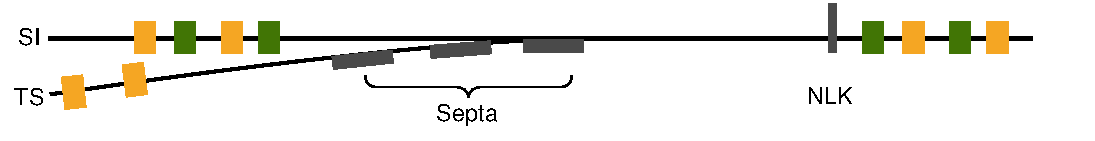
\includegraphics[width=\textwidth]{injection.pdf} 
    \begin{minipage}{0.49\textwidth}
        \begin{figure}
            \centering
        \end{figure}
        \begin{figure}
            \centering
            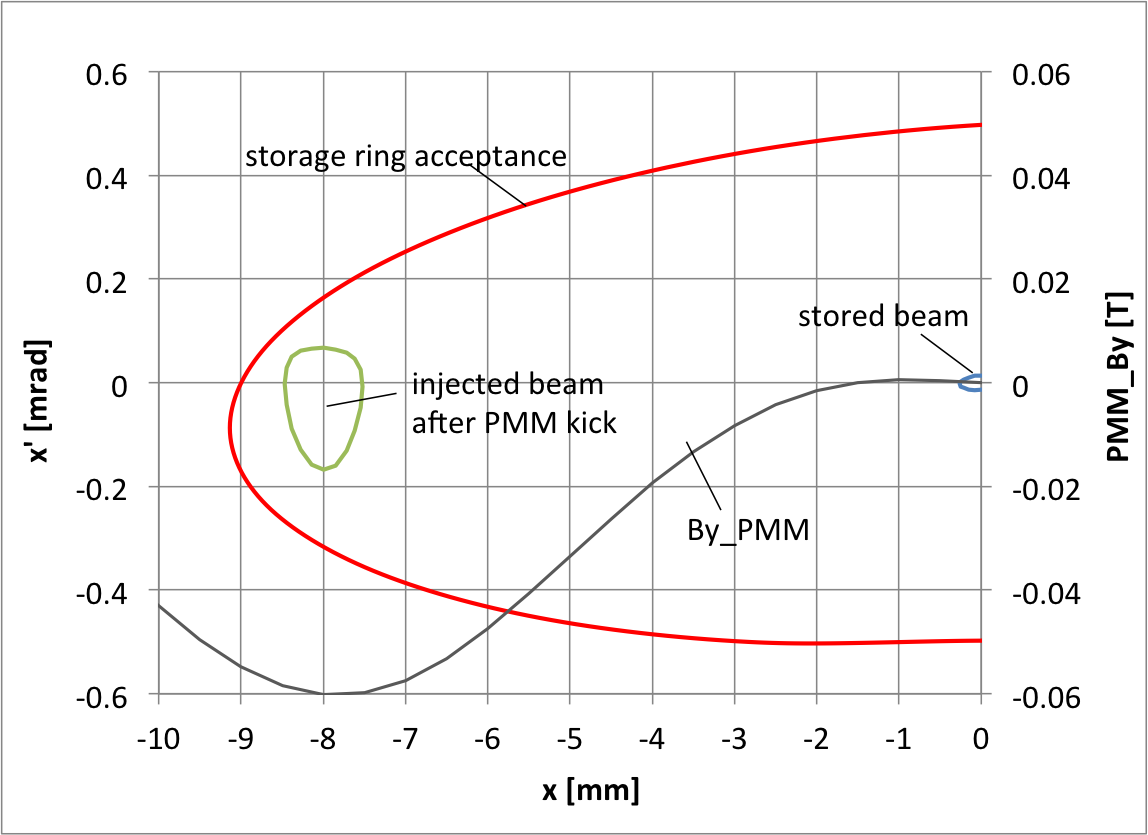
\includegraphics[width=\textwidth]{nlk_phase_space.png}
        \end{figure}
    \end{minipage}
    \begin{minipage}{0.49\textwidth}
        \begin{itemize}
            \item 100\% efficiency with a $x=-9~\unit{mm}$ DA 
            \item $88\pm8\%$ efficiency is observed
        \end{itemize}
    \end{minipage}

\end{frame}

\begin{frame}{RCDS optimization setup}
    \begin{minipage}{0.49\textwidth}
        \begin{itemize}
        \item objective function: avg. injection efficiency of 5 pulses @ $\unit{2~Hz}$
        \begin{itemize}
            \item beam at the DA border to reduce efficiency
        \end{itemize}
        \item available knobs: 21 sextupole families \begin{itemize}
            \item knobs $\in$ chromaticity response matrix nullspace (13, 17 knobs)
            \item 13 free knobs + 6 compensation knobs 
        \end{itemize}
        \end{itemize}
        \vfill

        \scriptsize
        More details:\\

        M. M. S. Velloso, L. Liu, F. de Sá, M. Alves, X. Resende, and X.
        Huang, “Online optimization of SIRIUS nonlinear optics”,
        \textit{presented at IPAC'23}, Venice, Italy, May 2023,
    \end{minipage}
    \begin{minipage}{0.49\textwidth}
        \centering
        SIRIUS sextupole families
        \begin{table}[]
            \begin{tabular}{cl}
            \hline
            achromatic & \begin{tabular}[c]{@{}l@{}}SFA0, SDA0, \\ SFB0, SDB0,\\ SDP0, SFP0\end{tabular}                                                                \\ \hline
            chromatic  & \begin{tabular}[c]{@{}l@{}}SDA1, SFA1, \\ SDA2, SFA2, \\ SDA3,\\ SDB1,\\ SDB2, SFB2, \\ SDB3, \\ SFP1, SDP1,\\ SFP2, SDP2,\\ SDP3\end{tabular} \\ \hline
            \end{tabular}
            \end{table}
        
        \vspace{0.5cm}
    \end{minipage}
\end{frame}
\begin{frame}{Tuning at $\nu_x = 49.08, \nu_y = 14.14$ (Working Point 1)}
    \begin{minipage}{0.55\textwidth}
        \begin{figure}
            \centering
            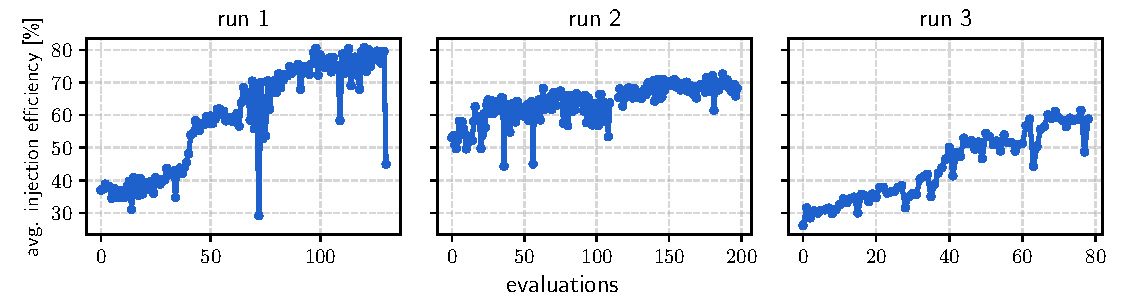
\includegraphics[width=\textwidth]{oldtunes_history.pdf}
            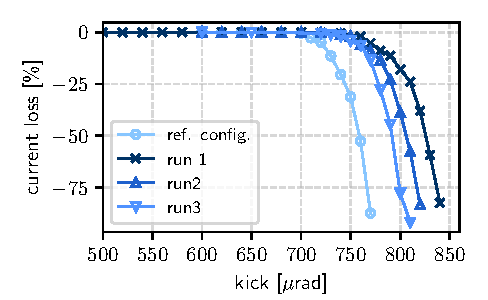
\includegraphics[width = 0.75\textwidth]{WEPL087_f1.pdf}
            \vfill
            \scriptsize
            \begin{table}[]
                \begin{tabular}{cc}
                \hline
                configuration & injection efficiency $[\%]$ \\ \hline
                ref-config    & $88\pm8$                    \\
                run 1         & $91\pm1$                    \\
                run 2         & $98\pm1$                     \\
                run 3         & $87\pm3$                     \\ \hline
                \end{tabular}
                \end{table}
        \end{figure}
    \end{minipage}
    \hfill
    \begin{minipage}{0.44\textwidth}
        \begin{figure}
            \centering
            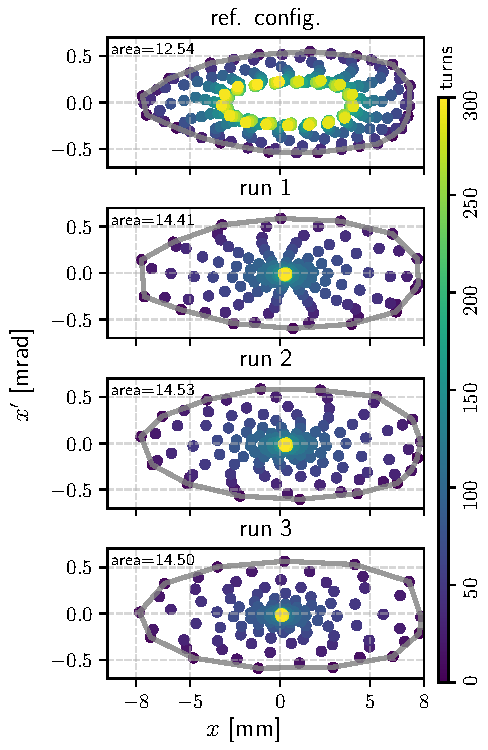
\includegraphics[height=0.9\textheight]{WEPL087_f2.pdf}
        \end{figure}
    \end{minipage}
\end{frame}
\begin{frame}{Tuning at $\nu_x = 49.20, \nu_y = 14.25$ (Working Point 2)}
    \begin{minipage}{0.55\textwidth}
        \begin{figure}
            \centering
            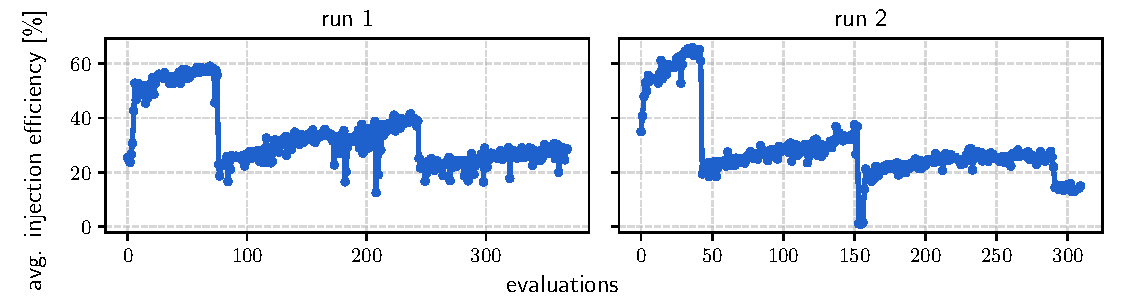
\includegraphics[width=\textwidth]{newtunes_history.pdf}
            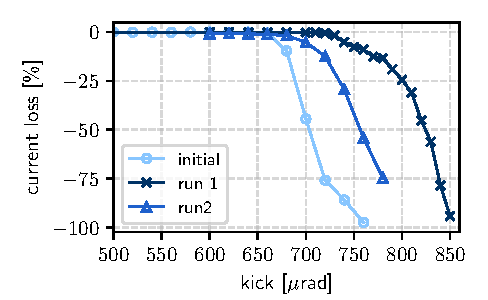
\includegraphics[width = 0.75\textwidth]{WEPL087_f3.pdf}
            \begin{table}[]
                \scriptsize
                \begin{tabular}{cc}
                \hline
                configuration & injection efficiency $[\%]$  \\ \hline
                non-optimized    & $51\pm1$                   \\
                run 1            & $79\pm3$                    \\
                run 2            & $65\pm1$                     \\ \hline
                \end{tabular}
                \end{table}
        \end{figure}
    \end{minipage}
    \hfill
    \begin{minipage}{0.44\textwidth}
        \begin{figure}
            \centering
            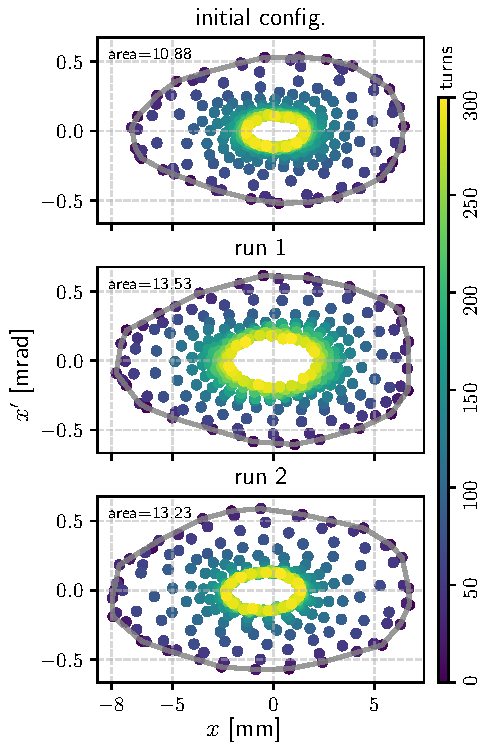
\includegraphics[height=0.9\textheight]{WEPL087_f4.pdf}
        \end{figure}
    \end{minipage}
\end{frame}
\begin{frame}{Tuning at $\nu_x = 49.16, \nu_y = 14.22$ (Working Point 3)}
    \begin{minipage}{0.55\textwidth}
        \begin{figure}
            \centering
            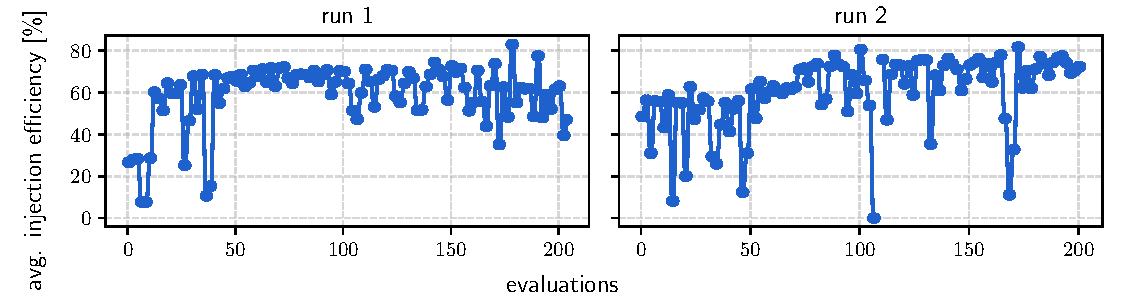
\includegraphics[width=\textwidth]{wp3_history.pdf}
            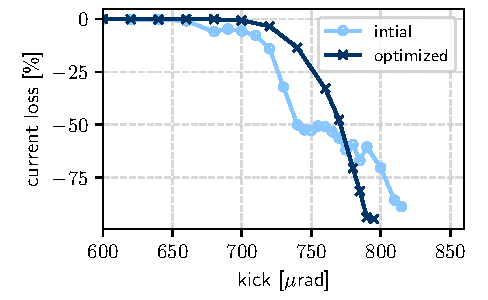
\includegraphics[width = 0.75\textwidth]{wp3_kick_resilience.pdf}
            \begin{table}[]
                \scriptsize
                \begin{tabular}{cc}
                \hline
                configuration & injection efficiency $[\%]$  \\ \hline
                non-optimized       & $-\pm1$                   \\
                optimied            & $93\pm3$                    \\ \hline
                \end{tabular}
                \end{table}
        \end{figure}
    \end{minipage}
    \hfill
    \begin{minipage}{0.44\textwidth}
        \begin{figure}
            \centering
            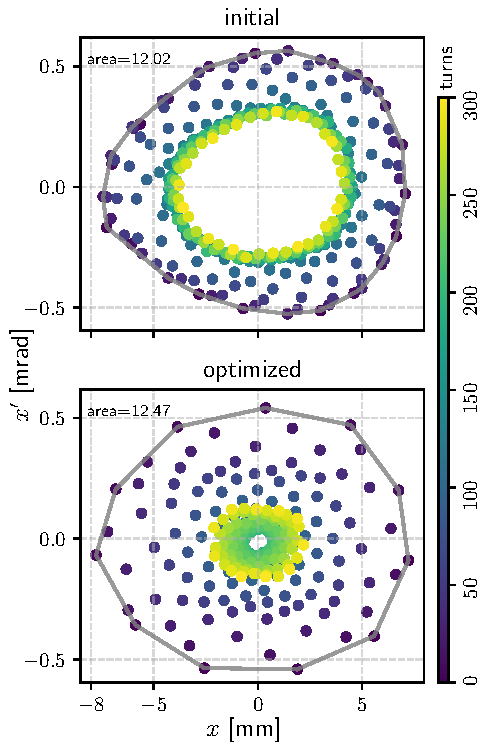
\includegraphics[height=0.9\textheight]{wp3_phase_space.pdf}
        \end{figure}
    \end{minipage}
\end{frame}

% \begin{frame}{Summary}
%     \begin{itemize}
%     \item Tuning was effective at optimizing injection efficiency
%     \item Some mysteries
%     \begin{itemize}
%         \item Larger kick resiliency $\centernot\implies$ larger phase portrait areas $\centernot\implies$ injection efficiency
%     \end{itemize}
%     \item A good sextupole setting was found in WP 3, which contributed for SIRIUS recent milestone of reaching $<1\% \sigma_x$ and $<4\% \sigma _y$ orbit stability in the horizontal and vertical, respectively
%     \end{itemize}
% \end{frame}

\section{Fast ORM Measruement}
\begin{frame}{Fast ORM Measurement}
    \begin{minipage}{0.44\textwidth}
        \begin{figure}
            \centering
            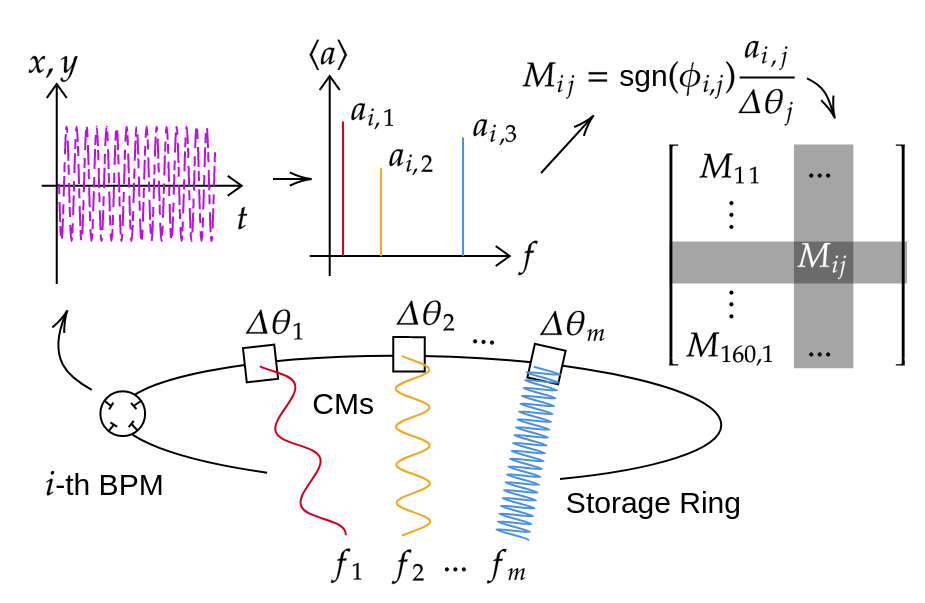
\includegraphics[width=\textwidth]{MOPOTK002_f1.png}
        \end{figure}
        \tiny
        M.M.S. Velloso, M.B. Alves, and F.H. de Sá,
   \textquotedblleft{Fast Orbit Response Matrix Measurement via Sine-Wave Excitation of Correctors at SIRIUS}\textquotedblright, in \emph{Proc. IPAC'22}, Bangkok, Thailand, Jun. 2022, pp. 425--428.
    \end{minipage}
    \begin{minipage}{0.55\textwidth}
        \begin{itemize}
            \scriptsize
            \item Fitting to $i$-th BPM data $u_i(t_j)$:
                \begin{equation*}
                    \begin{bmatrix}
                        \cos (2\pi f_{1} t_{1}) & \sin( 2\pi f_{1} t_{1}) & ... &\\
                        \cos (2\pi f_{1} t_{2}) & \sin (2\pi f_{1} t_{2}) & ...& \\
                        \vdots  & \vdots  & & \\
                        \cos (2\pi f_{1} t_{n}) & \sin (2\pi f_{1} t_{n}) & ... &
                        \end{bmatrix}\begin{bmatrix}
                            b_{i}{}_{1}\\
                            c_{i}{}_{1}\\
                            \vdots \\
                            b_{i}{}_{m}\\
                            c_{i}{}_{m}
                        \end{bmatrix} =\begin{bmatrix}
                            u_{i}( t_{1})\\
                            u_{i}( t_{2})\\
                            \vdots \\
                            u_{i}( t_{n})
                        \end{bmatrix}
                \end{equation*}
            \item Expected beam motion $$\Delta u_i(t)_n = \sum_j a_{i,j}\sin(2\pi f_j t_n + \phi_{i,j})$$
                \begin{equation*}
                    a_{i,j}=\sqrt{b^2_{i,j}+c^2_{i,j}}, \quad \phi_{i,j}=\text{atan}2(b_{i,j},c_{i,j})\in(-\pi,\pi]
                \end{equation*}
            \item ORM elements:
                \begin{equation*}
                    M_{ij}=\text{sgn}(\phi_{i,j})\frac{a_{i,j}}{\Delta \theta_j},
                \end{equation*}
        \end{itemize}
    \end{minipage}
\end{frame}
\begin{frame}{Measurements at SIRIUS storage ring and LOCO performance}
    \begin{minipage}{0.49\textwidth}
        \scriptsize
        SIRIUS BPMs-CMs circuit
        \begin{itemize}
            \item 160 BPM buttons
            \item $n_x = 120$ CHs, $n_y=160$ CVs, $n=n_x+n_y=280$ CMs
        \end{itemize}
        Measurment Procedure
        \begin{itemize}
            \item At each one of the \textbf{20 sectors},
            \begin{itemize}
            \scriptsize
            \item \textbf{6 CHs} $f_x = 3,  7, 13, 19, 29, 37\ \unit{Hz}$
            \item \textbf{8 CVs} $f_y = 5, 11, 17, 23, 31, 41, 47, 59\ \unit{Hz}$
            \item $\unit{5~\micro rad}$ strength, during $\unit{4~seconds}$.
            \end{itemize}
            \item  The complete measurement took around $2.5-3\ \unit{min}$.
        \end{itemize}
    AC- and DC-ORM signature correlation
    \begin{itemize}
        \scriptsize
        \item $\cos\theta_j = \vb{v}_{\text{AC}, j}\centerdot \vb{v}_{\text{DC}, j}/\norm{\vb{v}_{\text{AC}, j}}\norm{\vb{v}_{\text{DC}, j}}$
        \item avg $|1 - \cos\theta_j|\sim0.03\%$ for diagonal blocks and $\sim3\%$ for off-diagonal blocks
    \end{itemize}
    \end{minipage}
    \hfill
    \begin{minipage}{0.49\textwidth}
        \begin{figure}
            \centering
            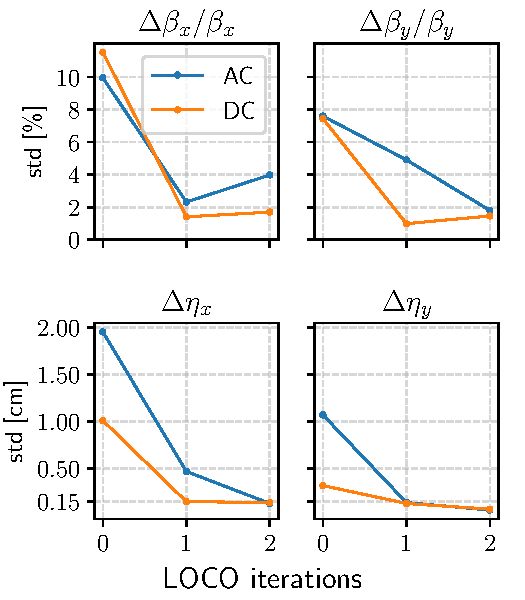
\includegraphics[width=\textwidth]{MOPOTK002_f5.pdf}
        \end{figure}
    \end{minipage}
\end{frame}
\begin{frame}[plain]
    Thank you!\\
    \vfill
    \url{matheus.velloso@lnls.br}\\
    \vfill
    M. M. S. Velloso is supported by the São Paulo Reseach Foundation via Grant \#2022/
    \begin{figure}
        \centering
        
\includegraphics[width=4cm]{fapesp.png}
    \end{figure}
    \begin{minipage}{0.49\textwidth}
        \begin{figure}
            
\includegraphics[width=5cm]{cnpem_lnls.png}
        \end{figure}
    \end{minipage}
    \begin{minipage}{0.49\textwidth}
        \begin{figure}
            
\includegraphics[width=5cm]{mcti.png}
        \end{figure}
    \end{minipage}
    \vfill
    
\end{frame}
\end{document}
